\documentclass[a4paper,12pt]{article}
\usepackage{graphicx}
\title{Chem 123L Lab \#2}
\date{January 24 2017}
\author{John Lawson\\partnered with Jett Chan\\TA: Lingzi Ma\\Section 003}
\begin{document}
\maketitle
\newpage

The goal of this lab was to successfully measure the concentration of alcohol in
a sample of wine provided. This is accomplished by reacting the alcohol present
in the sample with Potassium Dichromate, which produces free ${Cr}^{3+}$ ions in the
following reaction:


\begin{center}
 $3C_{2}H_{5}OH + 2K_{2}Cr_{2}O_{7} + 8H_{2}SO_{4} \rightarrow 2Cr_{2}(SO_{4})_{3} + 3CH_{3}COOH + 2K_{2}SO_{4} + 11H_{2}O$
\end{center}

The concentration of $Cr^{3+}$ ions produced can be assesed by optical tests
passing light through the solution, which in turn can be used to estimate the
alcohol concentration of the sample in question. For our experiment, several
known standards of alcohol were also tested in order to produce an expected
baseline for $Cr^{3+}$ produced based on alcohol content, which is then applied to
determine the alcohol content of our unknown.

The experimental procedure used for this experiment was outlined in the CHEM 123L
lab manual, experiment \#2. All steps were followed without deviation.
\newpage


\noindent

\title{Results}\\~\\

Unknown Wine Sample: \underline{D (2mL)}

\lbrack Dichromate Solution \rbrack: \underline{0.015 M in 5M $H_{2}SO_{4}$, 20mL}

Absorbance $\lambda$: \underline{575 nm}


\begin{center}
    \begin{tabular}{| l | l | l |}
    \hline
	Sample & Colour after heating & Measured Absorbance\\ \hline
	blank & orange & 0.000 \\ \hline
	2/8 (mL Ethanol/Water) & slightly lighter orange & 0.058\\ \hline
	4/6 (mL Ethanol/Water) & orange & 0.112\\ \hline
	6/4 (mL Ethanol/Water) & yellow to green & 0.178\\ \hline	
	8/2 (mL Ethanol/Water) & light green & 0.239\\ \hline    
    10/0 (mL Ethanol/Water) & light green & 0.278\\ \hline
    Diluted Wine Sample & light green (closer to 8/2 than 10/0) & 0.210\\ \hline    
    \hline
    \end{tabular}
\end{center}
\newpage
\begin{figure}
  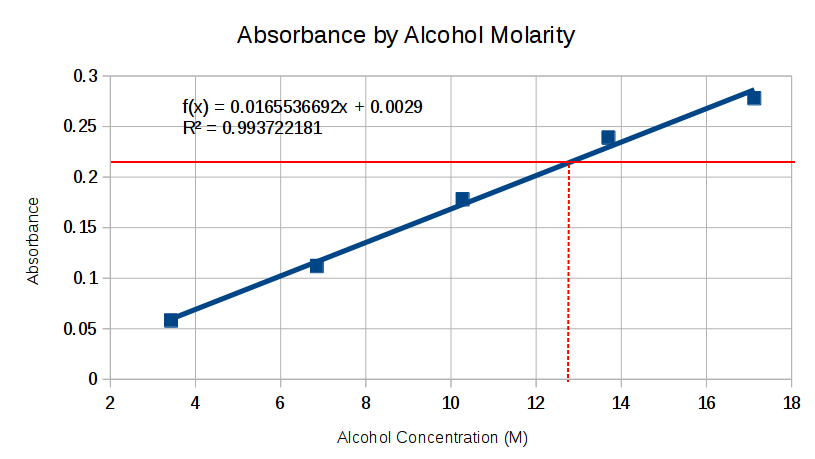
\includegraphics[width=\linewidth]{absorbbyEst.png}
  \caption{Absorbance by Molar Concentration, Estimate of unknown}
  \label{Absorbance by Molar Concentration, Estimate of unknown}
\end{figure}

Based on the best fit line, the concentration of the sample measured can
be estimated as 12.5 M, which is roughly equivalent to 73\% V/V
Since the sample was diluted from 1 mL to 100 mL for
measurement, the alcohol

\newpage
The foundations of the rigorous study of \emph{analysis}
were laid in the nineteenth century, notably by the
mathematicians Cauchy and Weierstrass. Central to the
study of this subject are the formal definitions of
\emph{limits} and \emph{continuity}.

Let $D$ be a subset of $\bf R$ and let
$f \colon D \to \mathbf{R}$ be a real-valued function on
$D$. The function $f$ is said to be \emph{continuous} on
$D$ if, for all $\epsilon > 0$ and for all $x \in D$,
there exists some $\delta > 0$ (which may depend on $x$)
such that if $y \in D$ satisfies
\[ |y - x| < \delta \]
then
\[ |f(y) - f(x)| < \epsilon. \]

One may readily verify that if $f$ and $g$ are continuous
functions on $D$ then the functions $f+g$, $f-g$ and
$f.g$ are continuous. If in addition $g$ is everywhere
non-zero then $f/g$ is continuous.

\end{document}
